\chapter{Wstęp}

Tutaj mają być jakieś słodkie ładne rzeczy o tym jaki to ten grafen jest super i
jak ładnie zrewolucjonizuje elektronikę i ją zmniejszy żeby spełnione było prawo
Moora.



	\section*{Quadratic equations}
			A quadratic equation is an equation of the form
			\begin{equation}
			\label{quad}
				ax^2 + bx + c = 0
			\end{equation}
			where \( a, b \) and \( c \) are constants and \( a \neq 0 \).
		\begin{wrapfigure}{r}{0.4\textheight}
		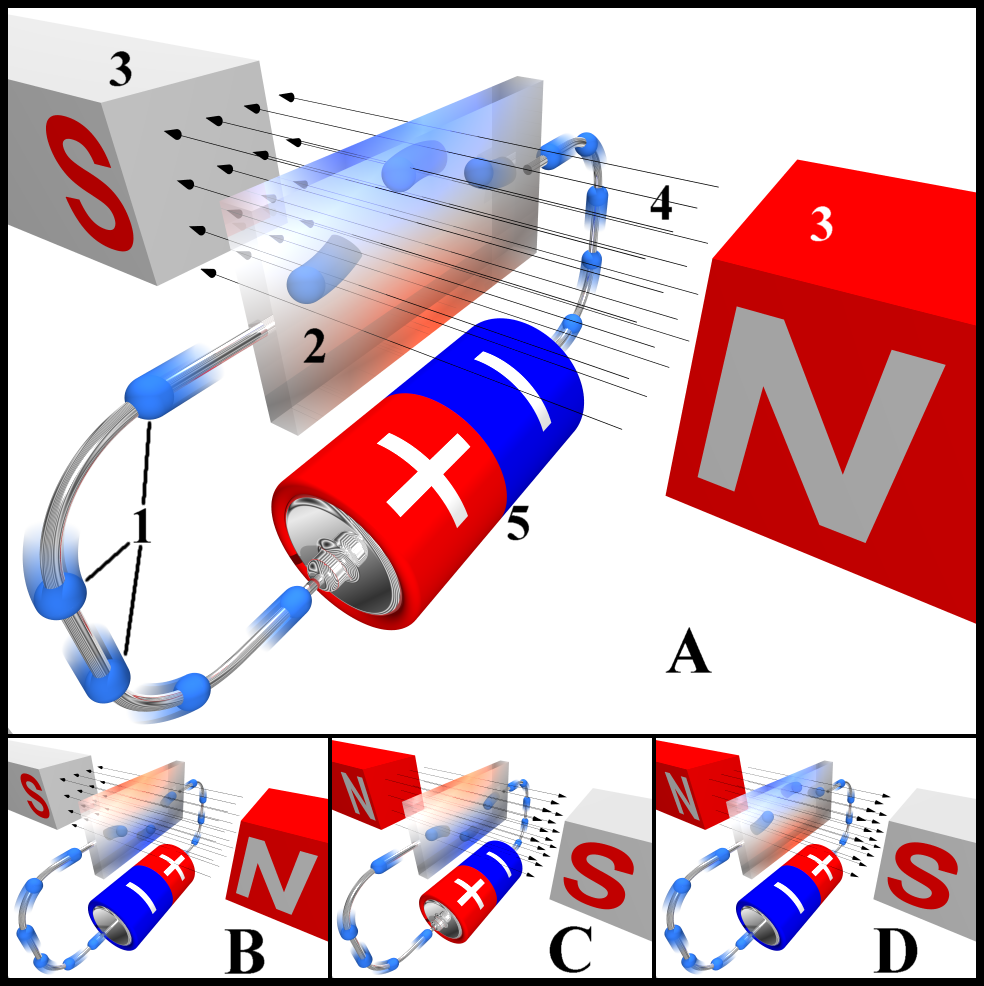
\includegraphics[width = 0.4\textheight]{./Rozdzial_1/Hall_effect.png}
		\caption{Klasyczny efekt halla}
		\label{klasyczny_hall}
		\end{wrapfigure}
\lipsum
